%%%%%%%%%%%%%%%%%%%%%%%%%%%%%%%%%%%%%%%%%%%%%%%%%%%%%%%%%%%%%%%%%%%%%%%%
% Plantilla TFG/TFM
% Escuela Politécnica Superior de la Universidad de Alicante
% Realizado por: Jose Manuel Requena Plens
% Contacto: info@jmrplens.com / Telegram:@jmrplens
%%%%%%%%%%%%%%%%%%%%%%%%%%%%%%%%%%%%%%%%%%%%%%%%%%%%%%%%%%%%%%%%%%%%%%%%

\chapter{Marco Teórico}
\label{marcoteorico}

El motor de videojuegos es el software encargado de que el desarrollador de videojuegos pueda programar estos sin tener que preocuparse por lo cómo se gestionan las entidades del juego, solo pensando en la lógica de las mecánicas, y demás aspectos del videojuego. En este \gls{tfg} voy a usar uno de creación propia, en base a las lecciones aprendidas en el curso de \citep{CursoMotorC++}, pero el mercado de motores de videojuegos es tan extenso que hay muchos que se podrían usar para el proyecto. Pero como la motivación del mismo es desarrollar las tecnologías de un videojuego desde cero, me he decidido por desarrollar el mío en el lenguaje C/C++ con el uso de algunas pocas librerías externas.

La \gls{ia} es el nombre que se utiliza para englobar todos los campos donde una máquina se comporta de manera inteligente, por lo tanto, hay que concretar más. El tema que se trata en este \gls{tfg} es el \gls{ml}, que busca dotar a las máquinas de la capacidad de aprendizaje, mediante el análisis de datos empíricos de una situación en la que se pretende predecir el resultado de un dato que no está presente dentro de esa muestra, y por supuesto, predecir al mismo tiempo los que sí lo están. 
\\
La parte común que converge en todos los tipos de aprendizaje es la siguiente: la máquina genera una función aleatoria, y esta función produce una salida en base a los datos de entrada que le han sido suministrados. Esta salida será, en la mayoría de los casos, errónea (dado que la función se ha generado de manera totalmente aleatoria), y no se parecerá en nada a lo que queremos que aprenda, así que según la forma de analizar y corregir este error de salida, se distinguen varios tipos de aprendizaje, los más comunes son:
\begin{description}
	\item[Supervisado:]  Los datos de entrada son proporcionados por el usuario que quiere entrenar al agente. Una vez obtenida la salida, comparamos esta salida real con la salida esperada, que realmente era la que debía haber generado, para obtener el error. Este tipo de entrenamiento se utiliza principalmente en tareas de etiquetado, como ejemplo más común tenemos la clasificación de un número escrito a mano, es decir, que un humano escriba un ocho y el agente entienda que es un ocho.
	\item[No supervisado:] A diferencia del anterior, no proporcionaremos datos de salida. Sirve para aprender a clasificar datos, según los patrones encontrados por el agente. En el ejemplo anterior, de clasificación de números, el agente podría identificar que dos números se parecen entre sí, pero no qué número es. La principal ventaja es que al no tener que proporcionar una salida, no es necesario que un humano etiquete los datos, así que es más sencillo obtener una gran cantidad de datos.
	\item[Reforzado:] A diferencia de los dos anteriores, sólo tenemos que indicar al agente cuál es el objetivo a conseguir, indicando qué acciones reportarán estímulos positivos para él, y cuáles estímulos negativos. No se proporcionan datos de entrada ni de salida, sino que los datos de entrada los obtiene probando acciones al azar en el medio, y la salida es la respuesta, el estímulo negativo o positivo.  Este tipo de aprendizaje es el más utilizado en videojuegos, ya que como son programas informáticos, es muy fácil simular una partida una cantidad muy grande de veces, sin embargo, el hecho de que el agente haya tomado una decisión correcta en ocasiones es muy difícil de determinar, así que se usan estímulos positicos como conseguir monedas o negativos como chocarse con una pared.
\end{description}

La unidad más básica de aprendizaje en el \gls{ml} es el perceptrón. Está inspirado en las neuronas del cuerpo humano, que reciben un impulso eléctrico desde varias entradas y deciden una salida booleana que es si continuar trasmitiendo la electricidad o no. 
Un perceptrón realmente, es lo mismo que una neurona, pero con una función de activación escalonada. Suma los valores de entrada, multiplicado por un peso previamente establecido, si supera un umbral dará un resultado, y si no lo supera, otro, por ejemplo: verdadero o falso, 1 o -1, etc.

\begin{figure}[h]
	\centering
	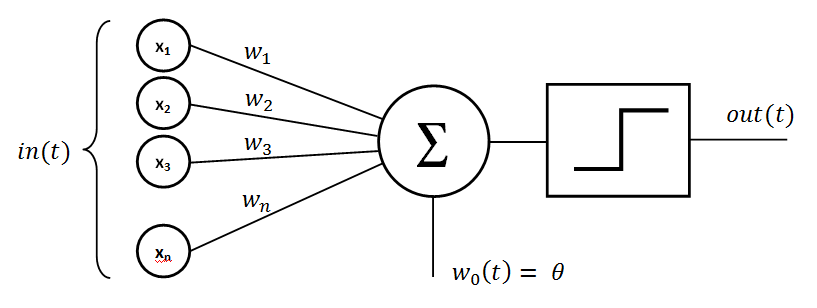
\includegraphics[width=15cm]{archivos/imagenes/perceptron.png}
	\caption{Perceptrón con entradas, pesos, y una salida escalonada. De wikimedia.org}
\end{figure}

Ha sido demostrado mediante estudios empírico-analíticos y teóricos, que con un correcto entrenamiento del perceptrón, evitando el sobreajuste\footnote{Conocido en la comunidad de \gls{ia} por su traducción en inglés, overfitting, ya que la mayoría de trabajos son hechos en este idioma.}, y proporcionando una cantidad suficiente de datos, que un solo perceptrón es capaz de separar los datos de cualquier problema que sea linealmente separable. Pudiendo entonces, mediante la sencilla implementación de un perceptrón, predecir patrones en cualquier campo con las condiciones mencionadas.

\section{Estado del Arte}
Entre los proyectos ya hechos con anterioridad a mi \gls{tfg} existen otros \gls{tfg} de compañeros de la \gls{ua}, entre los que cabe mencionar por su similitud, son los de \cite{tfg-ia-1}, \cite{tfg-ia-2}, \cite{tfg-ia-3} y \cite{tfg-ia-4}. Los cuales se pueden encontrar en los enlaces de la bibliografía.

Pero esto no es todo. Estos trabajos anteriormente mencionados tienen algo en común, a parte de pertenecer al mundo de la \gls{ia} y los videojuegos, todos están hechos utilizando un motor gráfico. Y como el objetivo de este \gls{tfg} no es solo crear el videojuego y la \gls{ia} sino también aprender el funcionamiento interno de cada uno de ellos, he necesitado seguir el curso de mi tutor \cite{CursoMotorC++} , en el cual explica y crea un motor gráfico desde cero, tan solo usando una librería de C para abrir ventanas \footnote{TinyPTC: descargable en el siguiente enlace \url{http://bit.ly/tinyPTC-UA19}} y otra en C++ para leer los sprites que se usarán en el juego\footnote{PicoPNG: descargable en el siguiente enlace \url{http://bit.ly/picoPNG-UA19}}.
\\
Como complemento a este motor gráfico que se explica en el curso, también usaré la librería Dear ImGui\footnote{ImGUI: descargable en el siguiente enlace \url{https://github.com/ocornut/imgui}}, que es una librería de código abierto usada por grandes empresas para la renderización de ventanas, texto, botones, y demás elementos necesarios para hacer una interfaz en un juego\footnote{Algunas de las empresas son Ubisoft, Supercell, Blizzard, etc. Todas en \url{https://github.com/ocornut/imgui/wiki/Software-using-dear-imgui}}. Así que a mitad del proyecto, cuando este esté avanzado y tenga que hacer las interfaces y los menús, cambiaré TinyPTC por OpenGL para poder usar Dear ImGui en el juego.

Además de los \gls{tfg} he decidido\footnote{Guiado por los conocimientos de mi tutor, Fran, que tiene los conocimientos y experiencia en el tema necesarios para aconsejarme los documentos en los que he de fijarme} realizar la lectura del libro \textit{Learning from Data: A Short Course} de \citefullauthor{LearningFromData}, un experto en el mundo de la Inteligencia Artificial. Un libro en el que da la iniciación, de forma teórica, al mundo del \gls{ml}, explicando el algoritmo más básico que es el perceptrón, con las fórmulas matemáticas y las propiedades estadísticas necesarias para entenderlo. Y las clases de la asignatura de Razonamiento Automático impartidas por mi tutor.

El \gls{ml} en videojuegos se puede usar para entrenar a un oponente del jugador, en cuyo caso es interesante definir varios niveles de dificultad. Puesto que entrenar a una máquina para que sea mejor que un humano en un juego es una tarea relativamente sencilla, la verdadera dificultad reside en que la máquina aprenda a jugar varios niveles, con los que se pueda ajustar al nivel de habilidad del jugador, de manera que siempre suponga un reto para el jugador batir a la máquina, pero que no sea tan extremadamente difícil que el jugador pierda las ganas de continuar jugando porque ha perdido el interés.
\\
Una segunda manera de usar el \gls{ml} es entrenando un agente para que bata los récords en un juego ya existente, es decir, que sustituya la posición del humano en el juego, de manera que consiga imitar o mejorar el comportamiento de un humano en el juego. Siendo el objetivo a batir un enemigo del juego, completar un mapa, o enfrentarse contra un humano. Esta segunda, es la manera que más se ha popularizado últimamente porque es algo más vistoso, y los ejemplos más conocidos son:
\begin{description}
	\item[MuZero:] Está desarrollada por DeepMind, empresa filial de  Google. Es capaz de ganar a cualquier humano jugando al Ajedrez, al Shogi y al Go.
	\item[AlphaStar:] También desarrollada por DeepMind. Es capaz de ganar a cualquier humano jugando al Star Craft, un juego de PC que trata de reunir recursos estratégicamente para combatir a tus enemigos.
	\item[Dino T-Rex:] Este no es una \gls{ia}, sino más bien un juego que se activa en Chrome cuando no tienes acceso a Internet. He decidido añadirlo en esta lista ya que al ser un juego tan conocido y sencillo, existen muchas personas que han decidido empezar programando su primera \gls{ia} con este, por ello, podemos encontrar muchos ejemplos simples de como entrenar a un agente en Internet.
	\item[Emergent Tool Use from Multi-Agent Interaction:] No se trata de ningún juego para humanos, pero es una herramienta desarrollada por OpenAI, una organización sin ánimo de lucro centrada en el desarrollo de \gls{ia} de código abierto. Trata de unos agentes que tienen que aprender a jugar al escondite, jugando dos contra dos, teniendo que aprender tanto los que pillan como los que son pillados a ganar. Estos agentes llegaron a desarrollar finalmente técnicas que explotan los fallos de las físicas del juego.\footnote{Para más información sobre el tema en el siguiente enlace se encuentra el paper \url{https://openai.com/blog/emergent-tool-use/}}
\end{description}